\chapter{Figures and Tables}\label{cha:figures}

With the chapter content ready, you can start adding figures and tables. This chapter first shows a single figure, then side-by-side figures, grid figures, traditional tables and three-line tables. On first use, paste the examples into your own chapter, confirm that it compiles, and only then replace the image paths, captions and data.

The template numbers everything automatically and by default puts the captions of figures and tables below them; to move them, follow the explanation in \ref{sec:caption}. The figures and numbers below are all layout samples; when you switch to your thesis, change the captions and notes with them.

\section{Inserting a Single Figure}

To insert a figure, put the image in the \code{figures/} folder and pass its path to \code{\fig}. The examples use the sample \code{figures/samples/architecture.png} that ships with the project; the path counts from the project root. The \code{0.6\linewidth} in square brackets sets the image width to sixty percent of the available text width; compile the example as it is first, then adjust the size to fit the image. When the brackets are omitted, the width defaults to \code{0.8\linewidth}.

\begin{lstlisting}[language=latex]
\fig[0.6\linewidth]{figures/samples/architecture.png}{Research framework}{fig:one}
\end{lstlisting}

The result is shown in \figref{fig:one}. With the default settings, the figure gets an automatically generated number and the text of the caption below it. The three braces are the image path, the caption and the label in that order; when you replace the image, change the path and the caption together. If you copy the example to add another figure, also change the last label \code{fig:one} so that every figure has its own name for use in the text; if you do not need to refer to it, leave it as \code{{}}.

\fig[0.6\linewidth]{figures/samples/architecture.png}{Research framework}{fig:one}

For other image options, the first bracket can take any width that \code{\includegraphics} understands, and for anything more elaborate skip \code{\fig}, use the standard \code{figure} environment and call \code{\includegraphics} yourself:

\begin{lstlisting}[language=latex]
\begin{figure}[htbp]
  \centering
  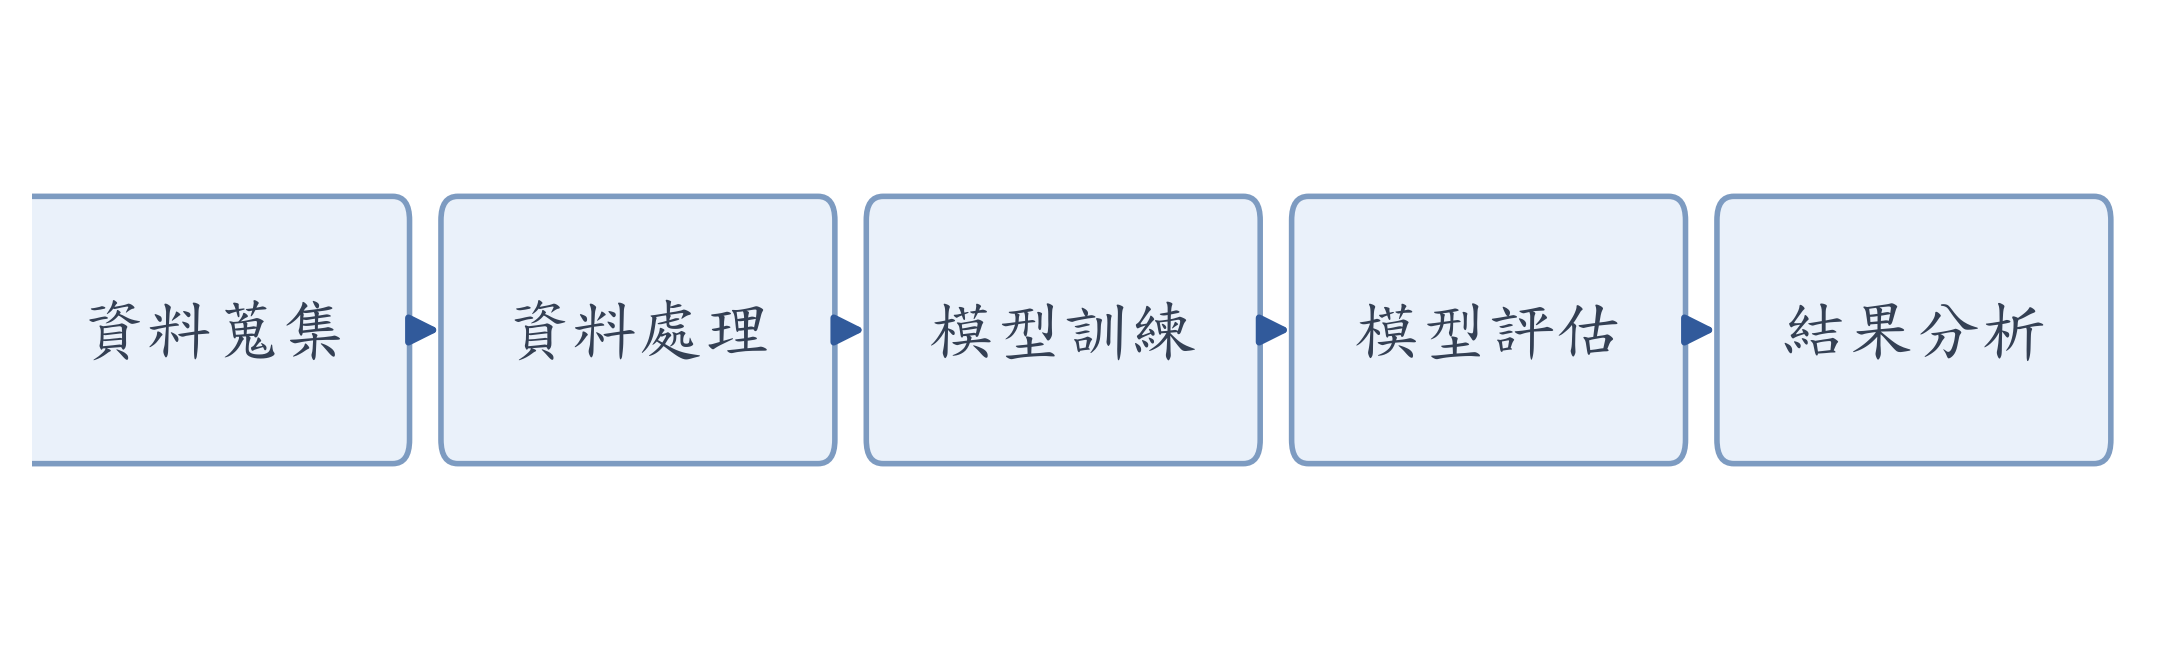
\includegraphics[width=0.6\linewidth,height=5cm,keepaspectratio]{figures/samples/architecture.png}
  \caption{Description}
  \label{fig:custom}
\end{figure}
\end{lstlisting}

\code{width} sets the displayed width; \code{0.6\linewidth} is sixty percent of the available text width, and a fixed length such as \code{8cm} also works. \code{height} sets the displayed height and, when omitted, follows the original proportions. Giving both stretches the image out of shape unless you add \code{keepaspectratio}, in which case the whole image keeps its proportions and is scaled to fit inside that area.

Other common options are \code{page} (which page of a multi-page PDF to insert, \code{1} by default) and \code{trim} with \code{clip} (cropping the edges). For the full list of parameters see the \href{https://ctan.org/pkg/graphicx}{documentation of graphicx}. A figure written the standard way does not follow \code{layout.caption-position.image}; to put its caption above, write \code{\caption} before \code{\includegraphics}.

\section{Side-by-side Figures}

To put two figures on the same row, use the \code{figrow} environment and give the path and sub-caption of each figure in order. The sub-captions are numbered \code{(a)}, \code{(b)} and so on automatically, and the whole group shares one figure number and one overall caption, so the list of figures shows only one entry. Here is how two figures are written:

\begin{lstlisting}[language=latex]
\begin{figrow}{Function graph comparison}{fig:row}
  \subfig{figures/samples/sin-x.pdf}{$\sin x$}
  \subfig{figures/samples/x-sin-x.pdf}{$x \sin x$}
\end{figrow}
\end{lstlisting}

\begin{figrow}{Function graph comparison}{fig:row}
  \subfig{figures/samples/sin-x.pdf}{$\sin x$}
  \subfig{figures/samples/x-sin-x.pdf}{$x \sin x$}
\end{figrow}

If you do not need sub-captions, leave the second brace empty. If the figures sit too close together after compiling, add \code{[gutter=2em]} after the environment name to widen the gap between the two columns, then check that the figures still have enough room.

\begin{lstlisting}[language=latex]
\begin{figrow}[gutter=2em]{Function graph comparison}{}
  \subfig{figures/samples/sin-x.pdf}{}
  \subfig{figures/samples/x-sin-x.pdf}{}
\end{figrow}
\end{lstlisting}

The \code{width} of side-by-side figures is relative to the width of each one's own column: with \code{[width=0.8]}, every figure takes eighty percent of its column. This is the value to lower when a figure needs to shrink; you need not edit the original image first.

\section{Grid Figures}

If there are more figures and you want several rows, use \code{figgrid} instead. \code{rows} sets the number of rows and \code{columns} the number of columns per row. The four figures below are placed with \code{rows=2} and \code{columns=2}, which lays them out in two rows from left to right and top to bottom. The sub-caption of each figure and the overall caption of the group are written just as for side-by-side figures.

\begin{lstlisting}[language=latex]
\begin{figgrid}[rows=2,columns=2,placement=auto]{Model predictions}{fig:grid}
  \subfig{figures/samples/a.pdf}{Linear model}
  \subfig{figures/samples/b.pdf}{Decision tree}
  \subfig{figures/samples/c.pdf}{Random forest}
  \subfig{figures/samples/d.pdf}{Neural network}
\end{figgrid}
\end{lstlisting}

\begin{figgrid}[rows=2,columns=2,placement=auto]{Model predictions}{fig:grid}
  \subfig{figures/samples/a.pdf}{Linear model}
  \subfig{figures/samples/b.pdf}{Decision tree}
  \subfig{figures/samples/c.pdf}{Random forest}
  \subfig{figures/samples/d.pdf}{Neural network}
\end{figgrid}

The four figures use the same synthetic training data: open circles are observed values, and solid black lines are each model's predictions. The data serve only to demonstrate the layout and are not experimental results of a real thesis. \code{placement=auto} lets \LaTeX{} treat the group as an ordinary float and decide, from the space left on the page, whether it stays in place or moves to a suitable position; when omitted it is \code{placement=none} and the group stays where it is written. \code{figrow} and \code{\fig} accept the same option, for example \code{\fig[width=0.6\linewidth,placement=auto]\{...\}}.

For two rows of three, set \code{rows=2,columns=3}. The figures are rearranged in the order they are given; the example below adds K-nearest neighbours and support vector regression after the first four models, filling all six cells. \code{rows} can be left out so that the number of rows grows with the number of figures; if you do specify a row count, the number of figures cannot exceed \code{rows * columns}. After adjusting, check that the text inside the figures is still legible; if it has become too small, reduce the number of columns.

\begin{lstlisting}[language=latex]
\begin{figgrid}[rows=2,columns=3]{Two rows, three columns}{fig:grid-2x3}
  \subfig{figures/samples/a.pdf}{Linear model}
  \subfig{figures/samples/b.pdf}{Decision tree}
  \subfig{figures/samples/c.pdf}{Random forest}
  \subfig{figures/samples/d.pdf}{Neural network}
  \subfig{figures/samples/e.pdf}{K-nearest neighbours}
  \subfig{figures/samples/f.pdf}{Support vector regression}
\end{figgrid}
\end{lstlisting}

The result is shown in \figref{fig:grid-2x3}:

\begin{figgrid}[rows=2,columns=3]{Two rows, three columns}{fig:grid-2x3}
  \subfig{figures/samples/a.pdf}{Linear model}
  \subfig{figures/samples/b.pdf}{Decision tree}
  \subfig{figures/samples/c.pdf}{Random forest}
  \subfig{figures/samples/d.pdf}{Neural network}
  \subfig{figures/samples/e.pdf}{K-nearest neighbours}
  \subfig{figures/samples/f.pdf}{Support vector regression}
\end{figgrid}

\section{Tables}

There are two ways to write a table: use the \code{tbl} environment when you need a rule around every cell, and the template's \code{tlt} environment for a three-line table, which has only the rules above and below the header and under the last row. The data are filled in the same way in both; only the look and the rules differ, so pick one according to your thesis or department rules.

\subsection{Traditional Tables}

When every cell needs a border, use the \code{tbl} environment. Its parameters are the caption, the label and the column format, and the column format works as in \code{tabular}: \code{ccc} means three centred columns, and adding \code{|} between columns draws vertical lines. Fill in the data from left to right and top to bottom, separate cells with \code{&}, end a row with \code{\\}, and draw a horizontal line with \code{\hline}.

\begin{lstlisting}[language=latex]
\begin{tbl}{Results (traditional table)}{tbl:traditional}{|c|c|c|}
  \hline
  Batch size & Accuracy (\%) & Training time (s) \\
  \hline
  32  & 91.2 & 48 \\
  64  & 92.8 & 31 \\
  128 & 92.1 & 22 \\
  \hline
\end{tbl}
\end{lstlisting}

\begin{tbl}{Results (traditional table)}{tbl:traditional}{|c|c|c|}
  \hline
  Batch size & Accuracy (\%) & Training time (s) \\
  \hline
  32  & 91.2 & 48 \\
  64  & 92.8 & 31 \\
  128 & 92.1 & 22 \\
  \hline
\end{tbl}

Adjacent cells can be merged. \code{\multicolumn{2}{c}{text}} lets one cell span two columns; in the three-column table below the ``Total'' row has only two cells, because ``100 samples'' already takes up the last two columns and there is no need to add a third. For a cell that spans two rows, use \code{\multirow{2}{*}{text}}; leave the occupied position in the next row empty.

\begin{lstlisting}[language=latex]
\begin{tbl}{Merged cells}{tbl:merged}{|c|c|c|}
  \hline
  Item & Training set & Test set \\
  \hline
  Samples & 80 & 20 \\
  \hline
  Total & \multicolumn{2}{c|}{100 samples} \\
  \hline
\end{tbl}
\end{lstlisting}

\begin{tbl}{Merged cells}{tbl:merged}{|c|c|c|}
  \hline
  Item & Training set & Test set \\
  \hline
  Samples & 80 & 20 \\
  \hline
  Total & \multicolumn{2}{c|}{100 samples} \\
  \hline
\end{tbl}

\subsection{Three-line Tables}

Unlike the traditional table that puts a border on every cell, the three-line table comes from the table conventions of \href{https://apastyle.apa.org/style-grammar-guidelines/tables-figures/tables}{APA style} and is most common in fields with many statistics, such as social science, education and psychology. Without the many vertical and horizontal lines the page looks cleaner, which is especially easy to read when whole columns are numbers. Most of the official regulations collected in \code{docs/} do not say which kind of rules a table should use; which one applies is usually the academic habit of the department or advisor rather than a school-wide rule, so it is worth confirming before you write.

A three-line table keeps only three horizontal rules: above and below the header and at the foot. With \code{tlt}, the top and bottom rules are drawn by the environment, and you write a \code{\midrule} yourself for the rule under the header. The data from before are reused below to make comparison easy.

\begin{lstlisting}[language=latex]
\begin{tlt}[notes={The values are layout samples.}]{Summary of results}{tbl:batch}{ccc}
  Batch size & Accuracy (\%) & Training time (s) \\
  \midrule
  32  & 91.2 & 48 \\
  64  & 92.8 & 31 \\
  128 & 92.1 & 22 \\
\end{tlt}
\end{lstlisting}

\begin{tlt}[notes={The values are layout samples.}]{Summary of results}{tbl:batch}{ccc}
  Batch size & Accuracy (\%) & Training time (s) \\
  \midrule
  32  & 91.2 & 48 \\
  64  & 92.8 & 31 \\
  128 & 92.1 & 22 \\
\end{tlt}

After the data are in, you can adjust column widths, alignment and the note under the table. The options in square brackets and the three arguments after them are:

\begin{tlt}{Common parameters of the three-line table}{tbl:tlt-args}{L{0.2\linewidth}L{0.7\linewidth}}
Parameter & Purpose and example \\
\midrule
Column format & \code{l}, \code{c}, \code{r} size by content; \code{L{4cm}} is a fixed-width left-aligned column, for longer text. \\
\code{width} & Option. Given a total width (e.g. \code{width=\linewidth}), the column format may use \code{X} to share the remaining width; when cells contain \code{\code}, use \code{L{...}} instead. \\
\code{thick}, \code{thin} & Options. Weight of the top and bottom rules and of the rule under the header; pass them to change one table only, or edit \code{\heavyrulewidth} at the top of the table section of \code{tw-thesis.sty} to change all tables. \\
\code{notes} & Option. A note under the table, at ninety percent of the body size. \\
\code{notes-label} & Option. The prefix of the note; ``Note.'' by default, and an empty \code{{}} removes it. \\
\end{tlt}

If there is so much data that a table does not fit on one page, \code{tlt} and \code{tbl} do not break across pages; use the \code{longtable} environment instead and add \code{\toprule}, \code{\midrule} and \code{\bottomrule} yourself; its \code{\endhead} repeats the header on every page. Afterwards check where the pages break and make sure readers can still tell the columns apart.

Three-line tables can merge cells too: in the example below, the ``Total'' row fills only two cells yet still occupies all three columns; compared with the traditional table above, the only difference is the style of the rules.

\begin{lstlisting}[language=latex]
\begin{tlt}{Merged cells in a three-line table}{tbl:tlt-merged}{ccc}
  Item & Training set & Test set \\
  \midrule
  Samples & 80 & 20 \\
  Total & \multicolumn{2}{c}{100 samples} \\
\end{tlt}
\end{lstlisting}

\begin{tlt}{Merged cells in a three-line table}{tbl:tlt-merged}{ccc}
  Item & Training set & Test set \\
  \midrule
  Samples & 80 & 20 \\
  Total & \multicolumn{2}{c}{100 samples} \\
\end{tlt}

The header itself can be grouped and set in two rows. When several columns fall into one category (for example ``Training set'' and ``Test set'' each split into accuracy and loss), split the header into two rows: the first uses \code{\multicolumn{2}{c}{...}} to span several columns and give the group name, and the second supplies the real name of each column; columns that need no grouping (such as ``Model'' on the far left) use \code{\multirow{2}{*}{...}} to span both header rows so no blank is left. To put a short rule under each group name, mark the range with \code{\cmidrule(lr){a-b}}, a command from the \code{booktabs} package, where \code{(lr)} leaves a little gap between the two short rules. To add a note to a single cell, put a superscript letter such as \code{\textsuperscript{a}} after its content and explain it in \code{notes}:

\begin{lstlisting}[language=latex]
\begin{tlt}[notes={\textsuperscript{a} Training stopped early (early stopping) and did not run the full number of epochs.}]{Grouped header}{tbl:tlt-grouped}{ccccc}
  \multirow{2}{*}{Model} & \multicolumn{2}{c}{Training set} & \multicolumn{2}{c}{Test set} \\
  \cmidrule(lr){2-3} \cmidrule(lr){4-5}
  & Accuracy (\%) & Loss & Accuracy (\%) & Loss \\
  \midrule
  Linear model & 88.1 & 0.42 & 85.3 & 0.51 \\
  Random forest & 96.4\textsuperscript{a} & 0.11 & 90.2 & 0.28 \\
\end{tlt}
\end{lstlisting}

\begin{tlt}[notes={\textsuperscript{a} Training stopped early (early stopping) and did not run the full number of epochs.}]{Grouped header}{tbl:tlt-grouped}{ccccc}
  \multirow{2}{*}{Model} & \multicolumn{2}{c}{Training set} & \multicolumn{2}{c}{Test set} \\
  \cmidrule(lr){2-3} \cmidrule(lr){4-5}
  & Accuracy (\%) & Loss & Accuracy (\%) & Loss \\
  \midrule
  Linear model & 88.1 & 0.42 & 85.3 & 0.51 \\
  Random forest & 96.4\textsuperscript{a} & 0.11 & 90.2 & 0.28 \\
\end{tlt}

In every row, the number of cells plus the columns each \code{\multicolumn} occupies must equal the number of columns in the column format: the first row is \code{1 + 2 + 2 = 5}, and the second leaves the first cell empty and fills four more; otherwise the table is laid out wrongly.

The three rules that \code{tlt} draws all come from the \code{booktabs} package and can be used directly inside a table:

\begin{tlt}{Rule commands of the three-line table}{tbl:booktabs}{L{0.3\linewidth}L{0.55\linewidth}}
Command & Where the rule goes \\
\midrule
\code{\toprule} & Top of the table; \code{tlt} draws it automatically \\
\code{\midrule} & Below the header, or between blocks \\
\code{\bottomrule} & Bottom of the table; \code{tlt} draws it automatically \\
\code{\cmidrule{a-b}} & Only over columns \code{a} to \code{b} (inclusive) \\
\end{tlt}

With \code{tlt}, only the \code{\midrule} below the header needs writing yourself; to add another rule in the middle of the data (for example to split it into two blocks of subtotals), just write one more \code{\midrule}. If you do not want \code{tlt} at all, you can also use the \code{tbl} environment and build the booktabs look yourself. For example:

\begin{lstlisting}[language=latex]
\begin{tbl}{Hand-built table with booktabs rules}{}{ccc}
  \toprule
  Item & Group 1 & Group 2 \\
  \midrule
  Mean & 91.2 & 88.5 \\
  Std. dev. & 3.1 & 4.2 \\
  \midrule
  Samples & \multicolumn{2}{c}{60} \\
  \bottomrule
\end{tbl}
\end{lstlisting}

The two numbers in \code{\cmidrule{a-b}} are column numbers counted from 1 and inclusive; for example the \code{\cmidrule(lr){2-3}} in the grouped-header example above means columns 2 to 3. The default rule weights are \code{0.08em} for \code{\toprule} and \code{\bottomrule} and \code{0.05em} for \code{\midrule} and \code{\cmidrule}.

The three rules of \code{tlt} can be made thicker too. To change only one table, pass the \code{thick} and \code{thin} options:

\begin{lstlisting}[language=latex]
\begin{tlt}[thick=0.14em]{Thicker top and bottom rules}{tbl:thick}{cc}
  Item & Value \\
  \midrule
  Example & 1 \\
\end{tlt}
\end{lstlisting}

\begin{tlt}[thick=0.14em]{Thicker top and bottom rules}{tbl:thick}{cc}
  Item & Value \\
  \midrule
  Example & 1 \\
\end{tlt}

Compare the top and bottom rules of \tblref{tbl:batch} to see the difference \code{thick} makes. To give all tables the same weight (including those built by hand with \code{\toprule}, \code{\midrule}, \code{\bottomrule} and \code{\cmidrule}), edit the lengths at the top of the table section of \code{tw-thesis.sty}:

\begin{lstlisting}[language=latex]
\setlength\heavyrulewidth{0.08em}   % \toprule, \bottomrule
\setlength\lightrulewidth{0.05em}   % \midrule, \cmidrule
\setlength\cmidrulewidth{0.05em}
\end{lstlisting}

\section{Cross-references}

To mention a figure or table in the text, first give it a label and then refer to it with \code{\ref}. Labels can be named freely, but must not repeat within the document. The earlier examples already carry \code{fig:grid} and \code{tbl:batch}, so you can use the following directly:

\begin{lstlisting}[language=latex]
The four sample figures are arranged as shown in \figref{fig:grid}.
See \tblref{tbl:batch} for the detailed numbers.
This chapter follows the rules of \ref{cha:layout}.
\end{lstlisting}

After compiling, the labels turn into the matching numbers: the four sample figures are arranged as shown in \figref{fig:grid}, see \tblref{tbl:batch} for the numbers, and this chapter follows the rules of \ref{cha:layout}. Section references show the full hierarchy, so \ref{sec:caption} shows the chapter and section numbers. All of these references are clickable and jump to the figure, table or section.

\code{\figref}, \code{\tblref} and \code{\lstref} put ``Figure'', ``Table'' and ``Listing'' in front of the number; the word comes from \code{strings:}. If you want only the number, use \code{\ref}. After figures or tables are added or moved, the template renumbers them and the references in the text follow, so you never edit ``Figure n'' or ``Table n'' by hand. Section headings can be referred to the same way; just add a label after the heading:

\begin{lstlisting}[language=latex]
\chapter{Layout Settings}\label{cha:layout}
\section{Margins and Paper}\label{sec:margin}
\end{lstlisting}

The wording of section references is set under \code{cross-ref:} in \code{config.yml}. \code{C} is the chapter number, \code{S} the section number and \code{B} the subsection number; only the numbers needed at the level of the label are shown. The default uses Chinese numerals and shows ``第C章'', ``第C章第S節'' or ``第C章第S節第B小節'' by level. To show \code{2}, \code{2.5} and \code{2.5.1} instead, change it to:

\begin{lstlisting}[language=yaml]
cross-ref:
  numbering: "1"
  chapter: "C"
  section: "C.S"
  subsection: "C.S.B"
\end{lstlisting}

To add words, use \code{{C}}, \code{{S}} and \code{{B}}, for example \code{"Ch. {C} Sec. {S}"}. The style affects only the section references in the text; it does not change headings, the table of contents, figures, tables, citations or page references, and appendices keep labels such as ``Appendix A''.

A Chinese character can follow a reference directly: write \code{see\ref{sec:caption}} and \LaTeX{} adds no extra space between them. Around punctuation, leave spaces as the sentence needs.

To put your own words in front of a reference, do not use \code{\figref}; write \code{Table~\ref{tbl:batch}} directly. This is a per-reference approach and changes only that one spot. If the prefix of ``Figure 1'' and ``Table 1'' in captions and in the lists also needs to change, start from the source, which is the \code{strings:} described in a later section, instead of rewriting each reference.

\section{Math and the List of Symbols}

To put a formula in a sentence, wrap it in \code{$...$}, for example \code{$E = m c^2$}. To display it on its own line, use \code{\[ ... \]}; to number it, use the \code{equation} environment instead. This is \LaTeX{}'s native math syntax; see the \href{https://ctan.org/pkg/amsmath}{documentation of amsmath} for the full set of symbols. The template already loads \code{amsmath} and \code{amssymb}.

\begin{lstlisting}[language=latex]
Inline formula $E = m c^2$, and a display formula:

\[
  \int_0^1 x^2 \,\mathrm{d}x = \frac{1}{3}
\]
\end{lstlisting}

After compiling, the inline formula $E = m c^2$ sits in the same paragraph as the text and the integral below stands on its own line:

\[ \int_0^1 x^2 \,\mathrm{d}x = \frac{1}{3} \]

To refer to a formula later, use an \code{equation} environment and add a label after the formula. The example below uses \code{eq:pythagoras} as the name, and referring works as for figures and tables; \code{\eqref} prints the parentheses as well:

\begin{lstlisting}[language=latex]
\begin{equation}\label{eq:pythagoras}
  a^2 + b^2 = c^2
\end{equation}

As shown in \eqref{eq:pythagoras}.
\end{lstlisting}

\begin{equation}\label{eq:pythagoras}
  a^2 + b^2 = c^2
\end{equation}

As shown in \eqref{eq:pythagoras}. The numbering rule of formulas is set by \code{config.yml}, so you never write \code{(1)} by hand; by default every formula is numbered continuously as \code{(1)}, \code{(2)}...; if your department wants numbering by chapter (for example formulas in Chapter 3 shown as \code{(3.1)}, \code{(3.2)}, restarting from \code{(4.1)} in Chapter 4), set this under \code{layout:} in \code{config.yml}:

\begin{lstlisting}[language=yaml]
layout:
  equation-numbering: "1"      # 1 | a | A | i | I | *
  equation-per-chapter: true   # true numbers as "chapter.count" and restarts every chapter
\end{lstlisting}

\code{equation-numbering} decides only the style of the running number and is written like \code{footnote-numbering}; the chapter number is always Arabic and does not depend on this setting.

If the thesis uses abbreviations or mathematical symbols repeatedly, collect them in the list of symbols among the front pages. Open \code{contents/front/denotation.tex}, keep the \code{denotation} environment, and fill in entries with the syntax below. Each entry starts with \code{\item}, with the symbol in square brackets and the full name or definition after it:

\begin{lstlisting}[language=latex]
\begin{description}
  \item[CNN] Convolutional Neural Network
  \item[$\eta$] learning rate
\end{description}
\end{lstlisting}

\section{Figure and Table Captions}

The words ``Figure'' and ``Table'' (圖 and 表 in a Chinese thesis) appear in captions, in the lists of figures and tables and in every reference in the text; they are set in one place, under \code{strings:} in \code{config.yml}, so you never change them one by one:

\begin{lstlisting}[language=yaml]
strings:
  figure: "插圖" # figure prefix of a Chinese thesis, "圖" by default
  figure-en: "Fig." # used when language: english, "Figure" by default
  table: "附表" # table prefix of a Chinese thesis, "表" by default
  table-en: "Tab." # used when language: english, "Table" by default
\end{lstlisting}

After changing them, recompile and every figure and table produced by \code{\fig}, \code{figrow}, \code{figgrid}, \code{tlt} and \code{tbl} takes the new prefix, and the lists of figures and tables and the text of \code{\figref} and \code{\tblref} follow. If only one figure or table needs to differ from the rest, use the standard \code{figure} environment and write the name you want yourself:

\begin{lstlisting}[language=latex]
\begin{figure}[htbp]
  \centering
  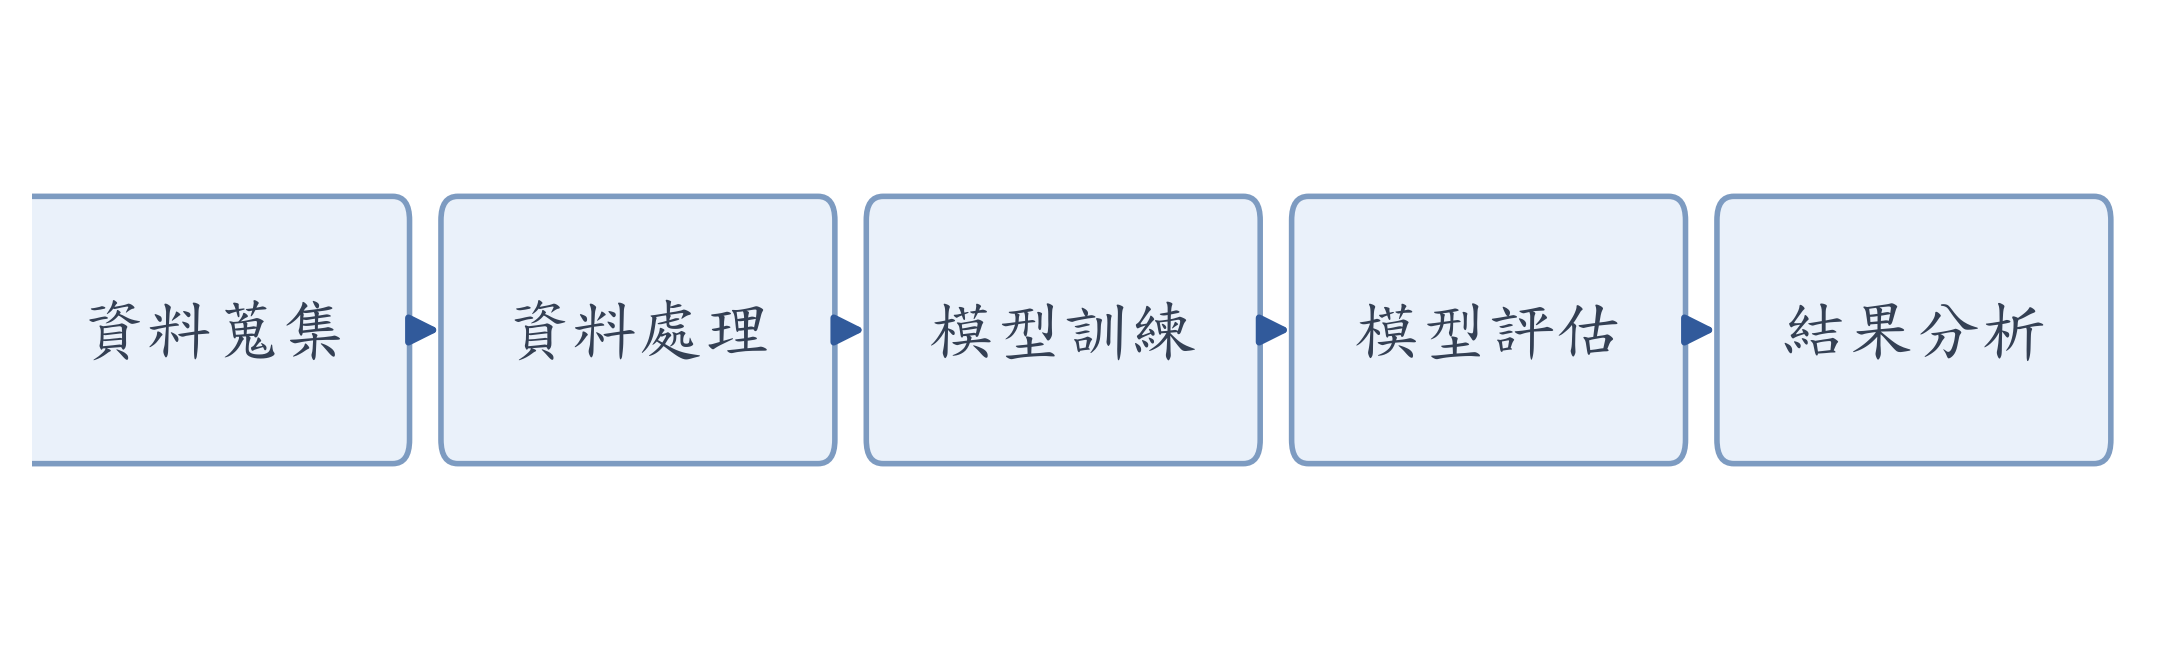
\includegraphics[width=0.6\linewidth]{figures/samples/architecture.png}
  \caption{Description}\label{fig:special}
\end{figure}
\end{lstlisting}

To make a figure show only its number without the prefix text, use \code{\caption*} for no numbering, or adjust \code{\captionsetup} of the \code{caption} package yourself; see the \href{https://ctan.org/pkg/caption}{documentation of caption}.

\section{Footnotes}

For additional remarks on figures and tables, the grouped-header example earlier put \code{\textsuperscript{a}} in a cell and explained it in \code{notes}; but that is a hand-made superscript, not a real footnote. For notes you can drop in anywhere in the text, numbered and typeset automatically by \LaTeX{}, use \code{\footnote{...}}; no other file needs editing, and the number, the superscript and the rule at the foot of the page are all handled for you:

\begin{lstlisting}[language=latex]
This point is somewhat disputed\footnote{Studies disagree on it.}, and later chapters return to it.
\end{lstlisting}

The result:

This point is somewhat disputed\footnote{Studies disagree on it.}, and later chapters return to it.

At the bottom of the page, numbering starts at 1 and keeps counting through the whole text, without resetting at page breaks. To cite the same note in several places, give a label to the first \code{\footnote}; you can then reuse the same number with \code{\footref} without creating a new footnote:

\begin{lstlisting}[language=latex]
First mention\footnote{The note text.}\label{fn:first}, and the second time\footref{fn:first}.
\end{lstlisting}

The number format and whether numbering restarts every chapter are both set under \code{layout:} in \code{config.yml}:

\begin{lstlisting}[language=yaml]
layout:
  footnote-numbering: "1"      # 1 | a | A | i | I | *
  footnote-per-chapter: false  # true restarts from 1 in each chapter
\end{lstlisting}

\code{footnote-numbering} is written like \code{outline.body-numbering} and the other numbering settings: \code{"1"} is Arabic numerals, \code{"a"} and \code{"A"} are letters, \code{"i"} and \code{"I"} are lower and upper case Roman numerals, and \code{"*"} is a star, then two stars and so on, which suits a thesis with few footnotes. \code{footnote-per-chapter} is \code{false} by default, so numbering runs on through the whole text; if your department wants each chapter to restart from 1, change it to \code{true}, with no need to reset the counter by hand at the start of every chapter.

With figures, tables, footnotes and formulas covered, the next chapter explains citing the literature, and code and appendices.
